% XCircuit output "schema_DC.tex" for LaTeX input from schema_DC.ps
\def\putbox#1#2#3#4{\makebox[0in][l]{\makebox[#1][l]{}\raisebox{\baselineskip}[0in][0in]{\raisebox{#2}[0in][0in]{\scalebox{#3}{#4}}}}}
\def\rightbox#1{\makebox[0in][r]{#1}}
\def\centbox#1{\makebox[0in]{#1}}
\def\topbox#1{\raisebox{-0.60\baselineskip}[0in][0in]{#1}}
\def\midbox#1{\raisebox{-0.20\baselineskip}[0in][0in]{#1}}
   \scalebox{0.8}{
   \normalsize
   \parbox{7.75521in}{
   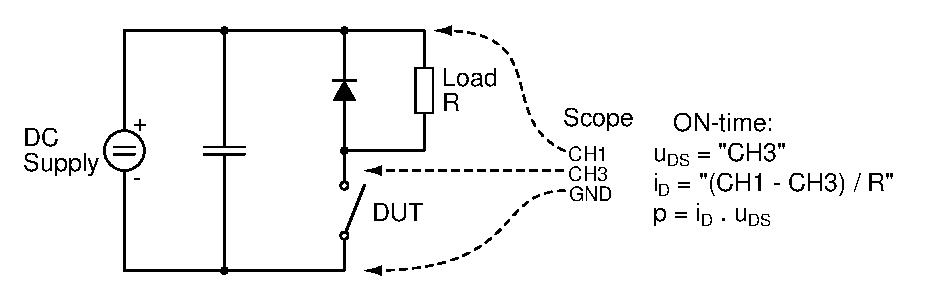
\includegraphics[scale=1.25]{schema_DC.ps}\\
   % translate x=751 y=391 scale 0.30
   \putbox{3.56in}{1.65in}{1.20}{Load}%
   \putbox{0.06in}{0.94in}{1.20}{Supply}%
   \putbox{0.98in}{1.27in}{1.20}{+}%
   \putbox{0.98in}{0.81in}{1.20}{-}%
   \putbox{2.98in}{0.52in}{1.20}{DUT}%
   \putbox{4.61in}{1.02in}{0.96}{CH1}%
   \putbox{4.61in}{0.86in}{0.96}{CH3}%
   \putbox{4.61in}{0.69in}{0.96}{GND}%
   \putbox{4.56in}{1.31in}{1.20}{Scope}%
   \putbox{5.31in}{1.02in}{1.20}{$u_{DS}$ = "CH3"}%
   \putbox{5.31in}{0.77in}{1.20}{$i_D$ = "(CH1 - CH3) / R"}%
   \putbox{5.48in}{1.27in}{1.20}{ON-time:}%
   \putbox{5.31in}{0.52in}{1.20}{$p = i_D \cdot u_{DS}$}%
   \putbox{3.56in}{1.44in}{1.20}{R}%
   \putbox{2.56in}{0.86in}{0.96}{D}%
   \putbox{2.56in}{0.27in}{0.96}{S}%
   \putbox{0.06in}{1.19in}{1.20}{DC Volt.}%
   } % close 'parbox'
   } % close 'scalebox'
   \vspace{-\baselineskip} % this is not necessary, but looks better
